\documentclass[paper=a4, fontsize=11pt]{scrartcl} % A4 paper and 11pt font size

\usepackage[T1]{fontenc} % Use 8-bit encoding that has 256 glyphs
\usepackage{fourier} % Use the Adobe Utopia font for the document - comment this line to return to the LaTeX default
\usepackage[english]{babel} % English language/hyphenation
\usepackage{amsmath,amsfonts,amsthm,amssymb} % Math packages

\usepackage{algorithm, algorithmic}
\renewcommand{\algorithmicrequire}{\textbf{Input:}} %Use Input in the format of Algorithm  
\renewcommand{\algorithmicensure}{\textbf{Output:}} %UseOutput in the format of Algorithm  

\usepackage{graphicx}
\usepackage{blindtext}
\usepackage{enumerate}
\usepackage{ulem} 
\usepackage{pdfpages}
\usepackage{multirow}

\usepackage{listings}
\lstset{language=Matlab}

\usepackage{lipsum} % Used for inserting dummy 'Lorem ipsum' text into the template

\usepackage{sectsty} % Allows customizing section commands
\allsectionsfont{\centering \normalfont\scshape} % Make all sections centered, the default font and small caps

\usepackage{fancyhdr} % Custom headers and footers
\pagestyle{fancyplain} % Makes all pages in the document conform to the custom headers and footers
\fancyhead{} % No page header - if you want one, create it in the same way as the footers below
\fancyfoot[L]{} % Empty left footer
\fancyfoot[C]{} % Empty center footer
\fancyfoot[R]{\thepage} % Page numbering for right footer
\renewcommand{\headrulewidth}{0pt} % Remove header underlines
\renewcommand{\footrulewidth}{0pt} % Remove footer underlines
\setlength{\headheight}{13.6pt} % Customize the height of the header

\numberwithin{equation}{section} % Number equations within sections (i.e. 1.1, 1.2, 2.1, 2.2 instead of 1, 2, 3, 4)
\numberwithin{figure}{section} % Number figures within sections (i.e. 1.1, 1.2, 2.1, 2.2 instead of 1, 2, 3, 4)
\numberwithin{table}{section} % Number tables within sections (i.e. 1.1, 1.2, 2.1, 2.2 instead of 1, 2, 3, 4)

\setlength\parindent{0pt} % Removes all indentation from paragraphs - comment this line for an assignment with lots of text

\newcommand{\horrule}[1]{\rule{\linewidth}{#1}} % Create horizontal rule command with 1 argument of height
\newcommand*{\dif}{\mathop{}\!\mathrm{d}}

\title{	
\normalfont \normalsize 
\textsc{Shanghai Jiao Tong University, UM-SJTU JOINT INSTITUTE} \\ [25pt] % Your university, school and/or department name(s)
\horrule{0.5pt} \\[0.4cm] % Thin top horizontal rule
\huge Technical Communication\\ HW6 \\ % The assignment title
\horrule{2pt} \\[0.5cm] % Thick bottom horizontal rule
}

\author{Yu Cang \quad 018370210001} % Your name

\date{\normalsize \today} % Today's date or a custom date

\begin{document}

\maketitle % Print the title

\section{Slides in \LaTeX}
	Please refer to ``../ex1/slide.pdf'' and ``../ex1/slide.tex''.
	
\section{Writting}
	\subsection*{First version}
		Turbulence combustion consists of complex flow and combustion phenomenon. Based on the model of flamelet, progress variable-flamelet model was developed for simulation of turbulence combustion. The progress variable was introduced to describe the complicated combustion phenomenon, such as local extinction and re-ignition. In my project, In order to exam the LES based on progress variable-flamelet model, I have been trying to apply this model to the simulation of diffusion jet flame, especially investigating the accuracy and availability of this model under the conditions of different Reynolds number, inflow profiles, and ignition approaches.
	\subsection*{Modified version}
		The research focuses on developing the progress variable flamelet model for simulating the turbulence combustion. There are some common phenomenon in turbulence combustion, e.g. local extinction and re-ignition, bringing great trouble to the simulation. And progress variable is very suitable to describe them. Large-eddy simulation(LES) is one of the most popular simulation methods in combustion field, and it is combined with variable-flamelet model for the simulation of diffusion jet flame in his project. The details include investigating the performance of this method under different combustion conditions.
	\subsection*{Final version}
		Focusing on developing the progress variable flamelet model for the simulation of turbulent combustion, the research is combining Large-eddy simulation(LES) with variable flamelet model, for diffusion jet flame simulation. Some complicated phenomenon in turbulence combustion, e.g. local extinction and re-ignition, bring great trouble to the simulation. And progress variable is developed to describe them. On the other hand, Large-eddy simulation is one of
		the most popular simulation methods in combustion field. To exam the availability of this combined model, a lot of numerical experiments under different conditions are proposed.
	
\section{Group Exercise}
	Please refer to Xuqing Zhou's submission, whose student ID is 118370910023.

\section{Leonardo da Vinci}
	This letter is excellent in terms of both contents and expressing skills. Generally, it is full of passion and confidence, which helps to make a positive atmosphere. \newline
	Introductions are split into 10 parts, with each focusing on a specific topic. This makes the general structure looks much clear. \newline
	In each part, active verbs and simple tense are used in the beginning to make it reads more powerful and reliable. Then, effects are vividly described. This is exactly the selling strategy "Sell the hole" does.\newline
	Besides, rhetoric words are used properly, which make it looks polite and suitable. All aspects like target readers, contends, time and conditions are well considered. I think it's a good job.
	
\section{IDEA survey}
	\begin{figure}[h]
		\centering
		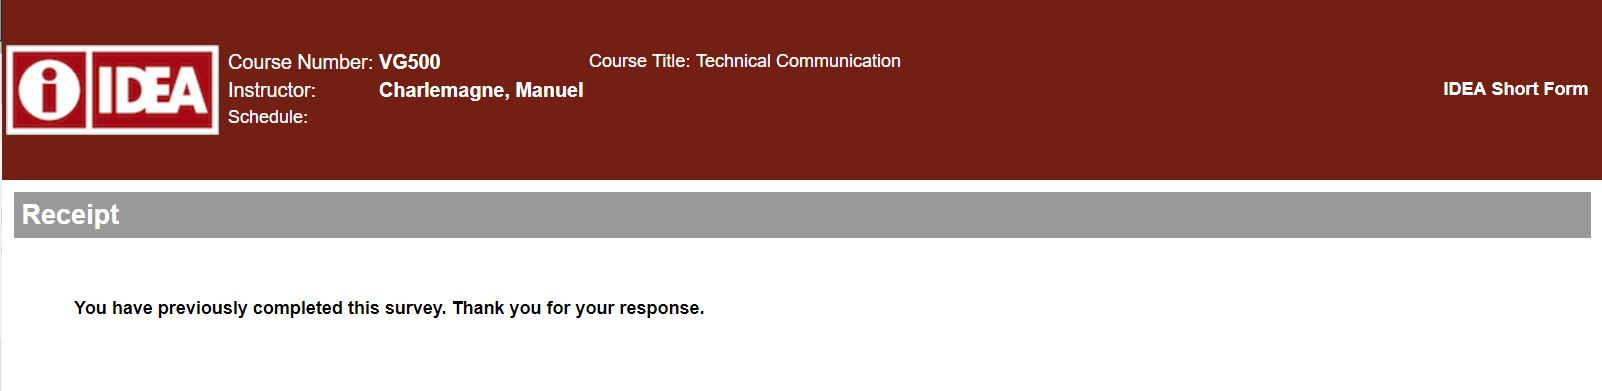
\includegraphics[width=\linewidth]{IDEA.jpg}
	\end{figure}
	
\end{document}
